\section{Malware Prediction}
\label{sec:predict}

\begin{figure}[t!]
\begin{center}
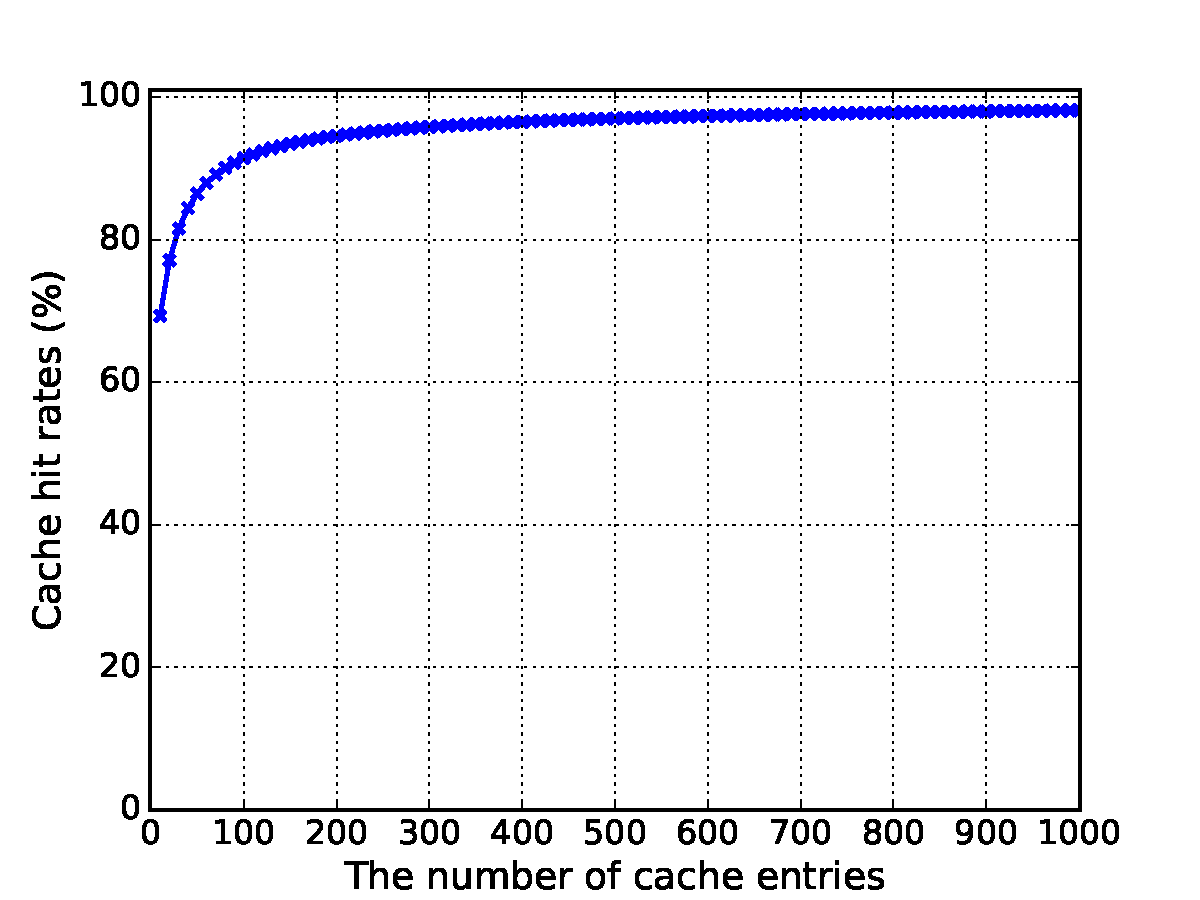
\includegraphics[width=3.0in]{figure/LRU}
\caption{Relation between cache hit rate and cache size.}
\label{fig:cache}
\end{center}
\end{figure}


\begin{figure}[t!]
\begin{center}
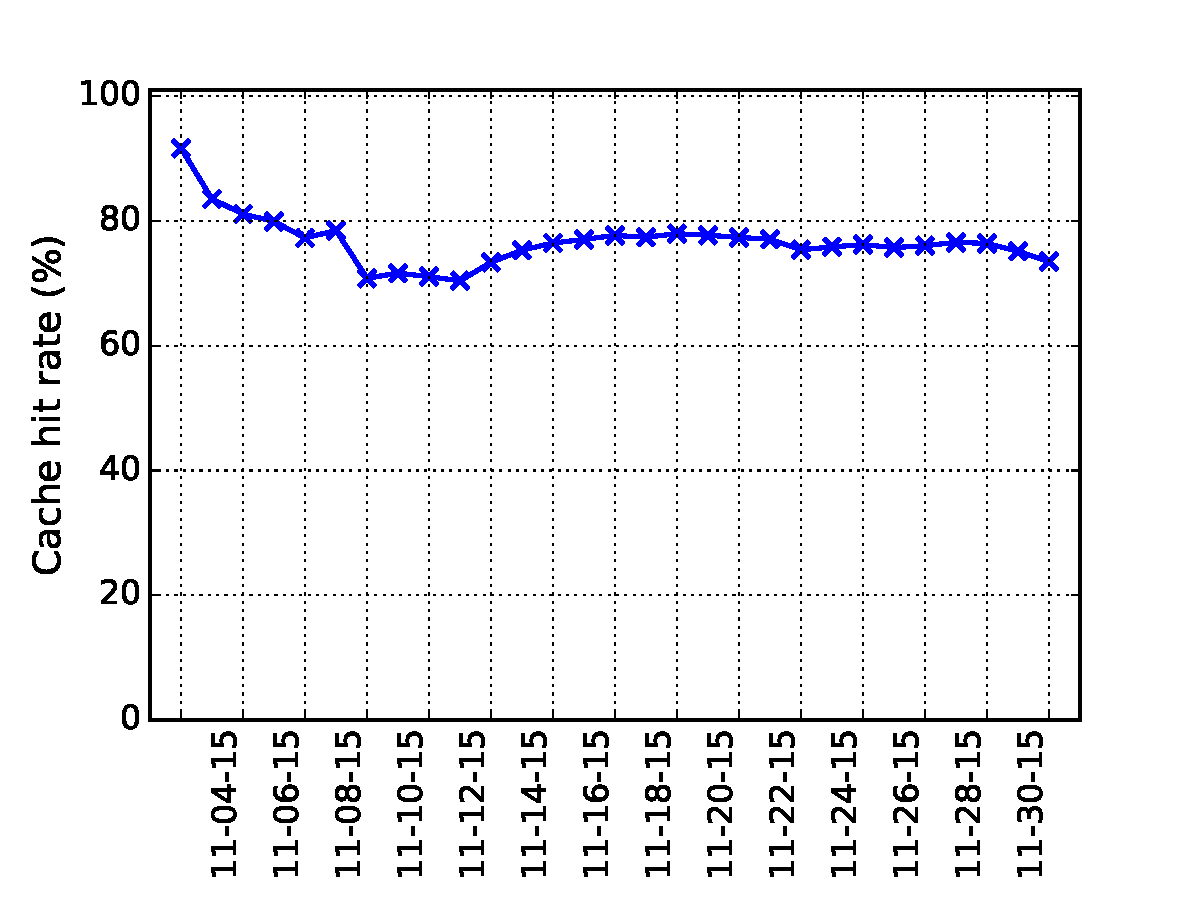
\includegraphics[width=3.0in]{figure/LRU_day}
\caption{Cache hit rate during per-day update.}
\label{fig:batchcache}
\end{center}
\end{figure}

Resources to combat malwares are limited. 
Any techniques that would allow antivirus vendors to focus their effort would be great. 
In this section, we build a stream mining algorithm which can predict malwares belong to which families would appear in the near future. 
The basic intuition behind our algorithm is that malwares do not appear uniformly across different family and time, but appear in bursts. 
We leverage cache mechanism~\cite{predicting} to predict which malwares would appear in the near future. 

We use N to represent the number of cache entries. 
One cache entry is used to save one malware family. 
We start our algorithm with empty cache. 
For a new malware submission, if the malware family is already in cache, 
we will change the sequence of cache entry, based on different cache eviction algorithm. 
If the new malware family is not in cache, we will create a new cache entry, 
and insert it into our cache. If cache is full, we need to evict some entry. 
There are many eviction policy. In this paper, we use LRU (least recently used). 

The hit rate is measured as: 

$$ \mbox{hit rate} = \dfrac{\mbox{\# of hits}}{\mbox{\# of hits + \# of misses}}$$

Figure~\ref{fig:cache} shows how cache hit rate changes with the number of cache sizes. 
Figure~\ref{fig:batchcache} shows how cache hit rate in each day, if we only update cache content at the end of each day. 

Discussion. 
There are other cache eviction policies we could try. 
We could explore how our malware cache would perform, if the block size is larger than one. We could explore how to conduct prefetch. 
We could also change the prediction granularity. 
The current granularity is malware family, and it is too coarse. 